\chapter{Designing for Injection Molding}\label{ch:molding}

\begin{tipbox}[When to Read This Chapter]
\textbf{Sprint~3 (CDR)}: Read the six DFM rules even if you are 3D printing your prototype. Good DFM practice (uniform walls, draft angles, radii) also produces better 3D prints and demonstrates design maturity at CDR. \textbf{Advanced/Entrepreneurial}: The tooling economics and mold classification sections are relevant if your team is considering a path from prototype to production.
\end{tipbox}


\vspace{1em}




\vspace{1em}


% ══════════════════════════════════════════════════════════════════════
\section{Injection Molding Fundamentals}
% ══════════════════════════════════════════════════════════════════════

\subsection{Process Overview}

Injection molding produces plastic parts by forcing molten thermoplastic into a precision steel mold under high pressure. The machine has two units: the \textbf{injection unit} (barrel, screw, heater bands, nozzle) melts pellets and injects them, and the \textbf{clamping unit} (platens, tie bars, hydraulic or toggle mechanism) holds the mold closed. Machines are rated by clamp force (tons) and shot size (oz or g).

The mold has two halves: the \textbf{cavity} (A-side, stationary, forms the outside/cosmetic surface) and the \textbf{core} (B-side, moving, forms the inside surface). The \textbf{parting line} is where the halves meet. Inside the mold, a \textbf{runner system} distributes melt from the nozzle to the gate, \textbf{cooling channels} extract heat, and \textbf{ejector pins\index{ejector pin}} push the part out.

\subsection{The Four-Phase Cycle}

\begin{figure}[htbp]
\centering
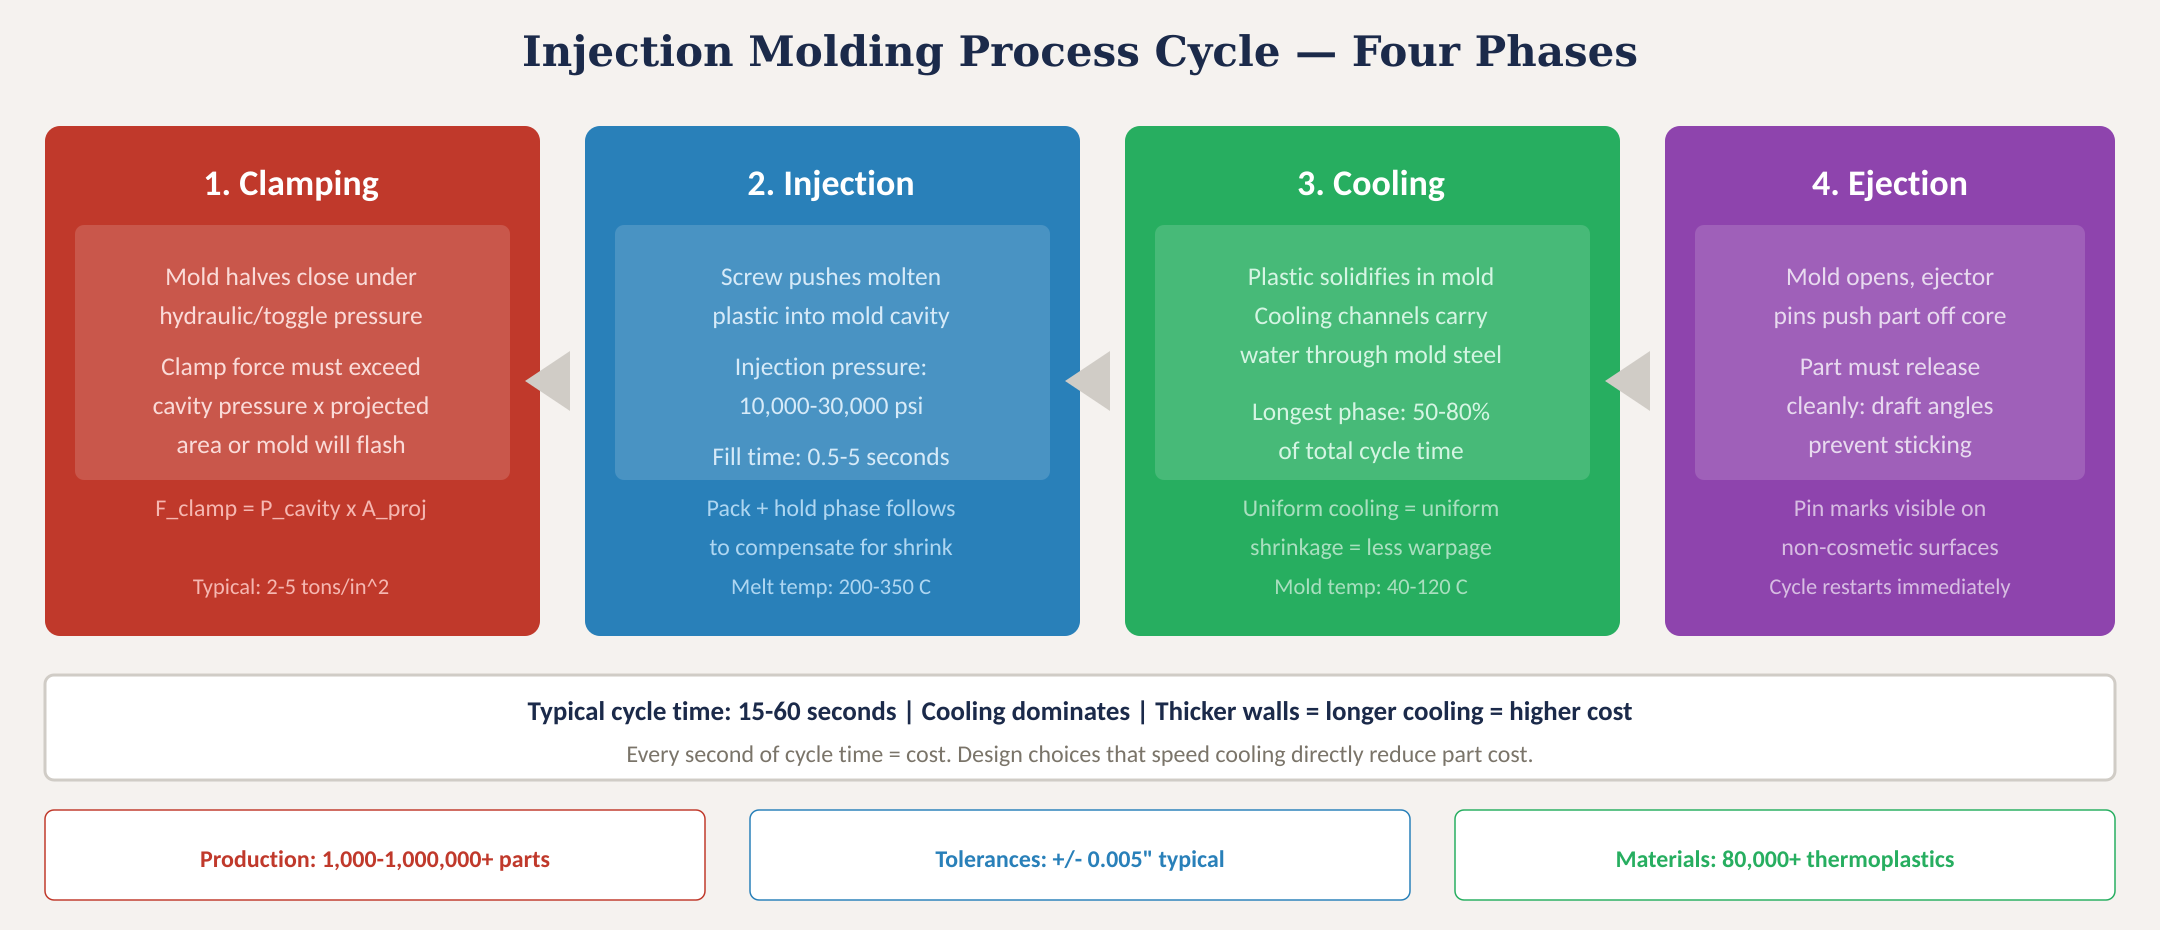
\includegraphics[width=\textwidth]{master_figs/fig_process_cycle.png}
\caption{Four-phase injection molding cycle with process parameters, timing, and production capabilities.}
\label{fig:cycle}
\end{figure}

\begin{enumerate}[leftmargin=1.5em]
  \item \textbf{Clamping}: Mold halves close under force. Required clamp force:
  \begin{equation}
    F_{\text{clamp}} = P_{\text{cavity}} \times A_{\text{projected}}
  \end{equation}
  Typical cavity pressures: 2--5~tons/in$^2$. A part with 10~in$^2$ projected area needs 20--50 tons of clamp force.

  \item \textbf{Injection}: The screw pushes molten plastic into the cavity at 10,000--30,000~psi. Fill time: 0.5--5~seconds. A \textbf{pack-and-hold} phase follows to compensate for volumetric shrinkage as the plastic cools. Without adequate packing, parts have sink marks\index{sink mark} and are undersized. Melt temperatures range from 200\,\degC{} (PE) to 350\,\degC{} (PC, nylon).

  \item \textbf{Cooling}: Plastic solidifies in the mold. This is the \textbf{longest phase}: 50--80\% of total cycle time. Cooling water flowing through channels in the mold steel extracts heat. \textbf{Uniform cooling = uniform shrinkage = minimal warpage.} Mold temperatures: 40--120\,\degC{} depending on material. Cooling time scales with the \emph{square} of wall thickness; doubling wall thickness quadruples cooling time.

  \item \textbf{Ejection}: Mold opens, ejector pins push part off the core. Part must have \textbf{draft angles\index{draft angle}} so it releases cleanly. Pin marks are visible on non-cosmetic (B-side) surfaces. The cycle restarts immediately.
\end{enumerate}

\begin{warningbox}[Cycle Time = Cost]
Typical total cycle: 15--60~seconds. Every additional second of cycle time increases part cost. Wall thickness is the primary driver; every millimeter of additional wall can add 5--15~seconds of cooling per cycle. Design the thinnest wall that meets structural and flow requirements.
\end{warningbox}


\subsection{Material Selection}
\label{sec:materials}

\begin{table}[htbp]
\centering\small
\begin{tabularx}{\textwidth}{l l X c l}
  \toprule
  \textbf{Material} & \textbf{Trade Names} & \textbf{Key Properties} & \textbf{Shrink} & \textbf{Common Uses} \\
  \midrule
  ABS & Cycolac & Good impact, easy to mold/paint, 80\,\degC{} & 0.5--0.7\% & Enclosures, LEGO \\
  PC & Lexan & High impact, optical clarity, 130\,\degC{}, UV-sensitive & 0.5--0.7\% & Lenses, phone cases \\
  PP & Pro-fax & Chemical resistant, living hinge\index{living hinge}, low cost & 1.0--2.5\% & Containers, caps \\
  Nylon (PA) & Zytel & High strength/stiffness, absorbs moisture & 0.8--1.5\% & Gears, connectors \\
  POM & Delrin & Low friction, dimensional stability, fatigue & 1.8--2.5\% & Gears, zippers \\
  PC/ABS & Bayblend & PC toughness + ABS processability & 0.5--0.7\% & Laptops, power tools \\
  PBT & Valox & Good electrical, chemical resistant & 1.5--2.0\% & Electrical connectors \\
  TPE/TPU & Santoprene & Flexible, rubber-like, overmoldable & 0.5--2.0\% & Grips, seals \\
  \bottomrule
\end{tabularx}
\caption{Common injection molding thermoplastics.}
\end{table}

\textbf{Selection criteria}: Match the \emph{cheapest} material that satisfies all of the following; mechanical loads (tensile, impact, flex), thermal environment (HDT, continuous use temperature, UL94 flammability), chemical exposure (solvents, UV, oils), aesthetics (gloss, texture, transparency, paintability), and processing (MFI, shrinkage, moisture sensitivity). Glass-fiber reinforcement increases stiffness 2--3$\times$ but reduces impact and abrades the mold.

\begin{tipbox}[Shrinkage Matters]
When hot plastic cools it contracts. The mold cavity is cut \emph{larger} than the finished part by the shrinkage factor. High-shrinkage materials (PP at 1--2.5\%) require more generous tolerances than low-shrinkage materials (ABS at 0.5--0.7\%). Crystalline polymers (PP, nylon, POM) shrink more than amorphous ones (ABS, PC, PS).
\end{tipbox}


% ══════════════════════════════════════════════════════════════════════
\section{Design for Manufacturing (DFM) Rules}
\label{sec:dfm}
% ══════════════════════════════════════════════════════════════════════

\begin{figure}[htbp]
\centering
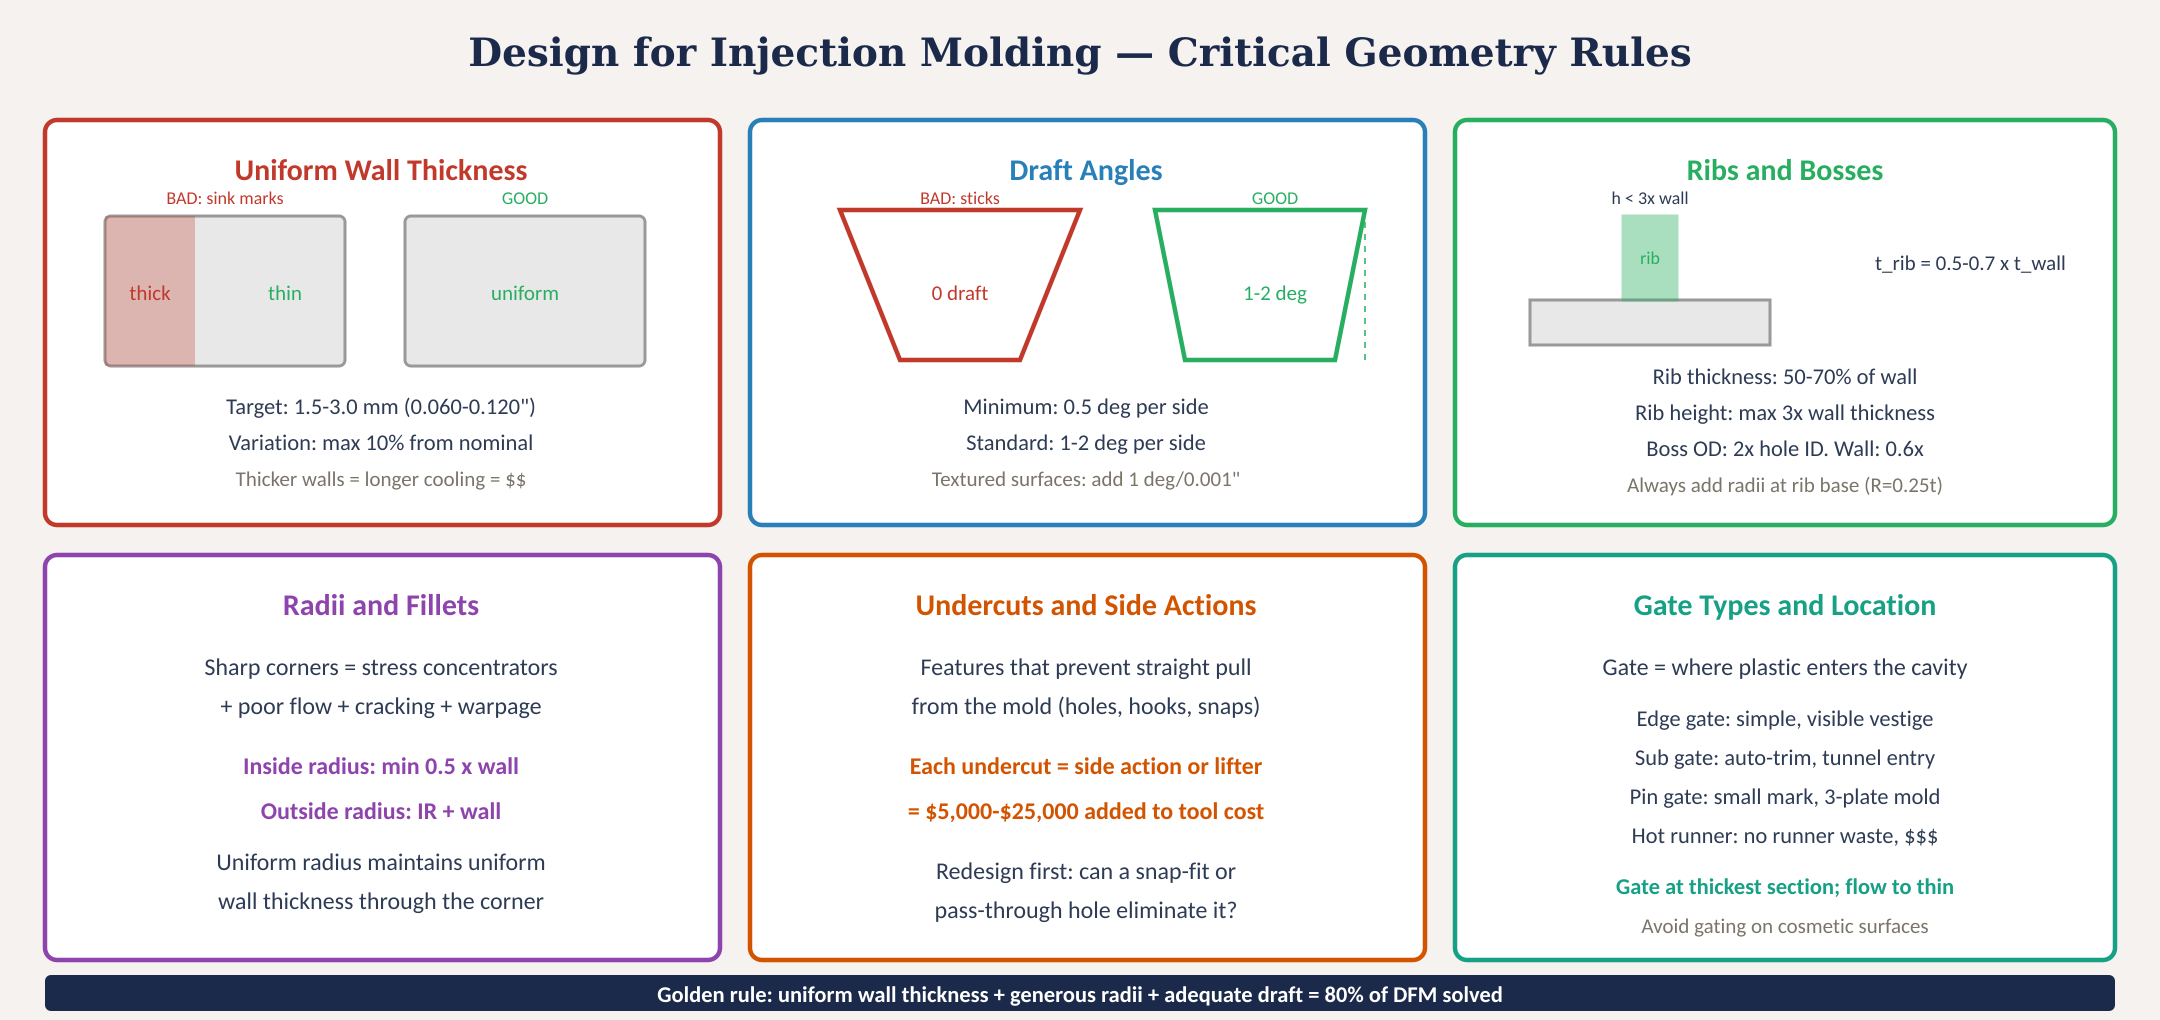
\includegraphics[width=\textwidth]{master_figs/fig_dfm_rules.png}
\caption{Six critical DFM geometry rules: wall thickness, draft angles, ribs/bosses, radii, undercuts, and gate location\index{gate location (mold)}.}
\label{fig:dfm}
\end{figure}

\subsection{Rule 1: Uniform Wall Thickness}

The single most important design parameter. Wall thickness drives cycle time (cooling $\propto t^2$), material usage, shrinkage uniformity, and defect susceptibility.

\textbf{Recommended ranges}: ABS: 1.5--3.5\,mm. PC: 1.5--3.5\,mm. PP: 0.8--3.0\,mm. Nylon: 1.0--3.0\,mm. POM: 1.0--3.0\,mm.

\textbf{Uniformity}: Variation $<$10\% of nominal. Where transitions are unavoidable, use gradual tapers at a 3:1 length-to-thickness-change ratio. Abrupt steps cause differential shrinkage, sink marks, and stress concentrations.

\textbf{Coring out}: Replace solid thick sections with thin uniform shells reinforced by ribs. A ribbed 2\,mm wall is stiffer than a solid 4\,mm wall, cools in one-quarter the time, and uses half the material.

\subsection{Rule 2: Draft Angles}

Draft is the slight taper on walls parallel to the mold opening direction that allows the part to release.

\begin{itemize}[nosep,leftmargin=1.5em]
  \item Minimum: \ang{0.5} per side (tight tolerance applications).
  \item Standard: \ang{1}--\ang{2} per side (recommended).
  \item Textured surfaces: add \ang{1} per 0.001\,in (0.025\,mm) of texture depth.
  \item Core side often needs more draft than cavity side (part shrinks onto core).
\end{itemize}

\begin{warningbox}[Zero-Draft = Stuck Parts]
Zero-draft vertical walls are the \#1 student DFM error. Without draft, the part grips the core, ejector pins push through the wall, and the mold wears rapidly. Apply draft to \emph{all} surfaces parallel to the pull direction; including internal ribs, bosses, and walls.
\end{warningbox}

\subsection{Rule 3: Ribs and Bosses}

Ribs add stiffness without mass; bosses provide screw/insert mounting points.

\subsubsection{Rib Proportions}
\begin{itemize}[nosep,leftmargin=1.5em]
  \item Thickness: 50--70\% of adjoining wall (thicker $\to$ sink marks on opposite surface).
  \item Height: max $3\times$ wall thickness (taller $\to$ fill and ejection problems).
  \item Draft: min \ang{0.5} per side (\ang{1} preferred).
  \item Spacing: min $2\times$ wall thickness between ribs.
  \item Base radius: 0.25--0.5 $\times$ wall thickness.
  \item Multiple thin ribs outperform one thick rib.
\end{itemize}

\subsubsection{Boss Proportions}
\begin{itemize}[nosep,leftmargin=1.5em]
  \item OD: 2.0--2.5 $\times$ screw/insert hole ID.
  \item Wall: 0.6 $\times$ nominal wall thickness.
  \item Freestanding bosses: connect to nearest wall with a rib.
  \item Height: max 2.5 $\times$ OD.
  \item For heat-set brass inserts: hole ID per insert manufacturer specification.
\end{itemize}

\subsection{Rule 4: Radii and Fillets}

Sharp inside corners create stress concentrations (up to $3\times$ at zero radius), impede melt flow, and cause sink marks.

\begin{itemize}[nosep,leftmargin=1.5em]
  \item Inside radius: min $0.5\times$ wall (1$\times$ preferred).
  \item Outside radius: inside radius $+$ wall thickness.
  \item This maintains uniform wall thickness through the corner.
  \item Apply radii to \emph{every} inside corner without exception.
\end{itemize}

\subsection{Rule 5: Undercuts}

Any feature preventing straight-pull mold separation; side holes, snap hooks, internal threads, louvers. Each undercut requires a side action (cam, lifter, or collapsing core), adding \$5,000--\$25,000 to tooling cost.

\textbf{Always redesign first}: Can a pass-through hole replace a blind side hole? Can a snap-fit be oriented along the pull direction? Can an internal thread become a heat-set insert installed after molding?

\subsection{Rule 6: Gate Location}

The gate is where plastic enters the cavity.

\begin{itemize}[nosep,leftmargin=1.5em]
  \item \textbf{Place at the thickest section} so melt flows from thick to thin (ensures adequate packing).
  \item \textbf{Never gate on a cosmetic surface}; the gate vestige is always visible.
  \item Gate types: edge gate (simple, visible mark), sub gate (auto-trimmed), pin gate (small mark, 3-plate mold), hot runner (no runner waste, highest tooling cost).
  \item Flow simulation (Moldflow) predicts fill pattern and weld line\index{weld line} locations.
\end{itemize}


\begin{quickrefbox}[Quick Reference: Six DFM Rules at a Glance]
\begin{table}[H]\centering\small
\begin{tabularx}{\linewidth}{c l X c}
\toprule
\textbf{\#} & \textbf{Rule} & \textbf{Key Values} & \textbf{Consequence of Violation} \\
\midrule
1 & Uniform wall & ABS/PC: 1.5--3.5\,mm; variation $<$10\% & Sink marks, warpage \\
2 & Draft angles & $\geq$\ang{1}/side; +\ang{1} per 0.001'' texture & Part stuck in mold \\
3 & Ribs \& bosses & Rib = 50--70\% of wall; height $\leq 3\times$ wall & Sink marks, voids \\
4 & Radii & Inside $\geq 0.5\times$ wall; outside = inside + wall & Stress cracks \\
5 & Undercuts & Avoid or use side-actions/collapsing cores & Mold cost doubles \\
6 & Gate location & Thickest section; flow toward thin; balanced & Short shots, weld lines \\
\bottomrule
\end{tabularx}
\end{table}
\end{quickrefbox}


% ══════════════════════════════════════════════════════════════════════
\section{Common Defects}
\label{sec:defects}
% ══════════════════════════════════════════════════════════════════════

Every defect has a root cause in part geometry, material, or process. Good design eliminates most defects before the mold is ever cut.

\begin{figure}[htbp]
\centering
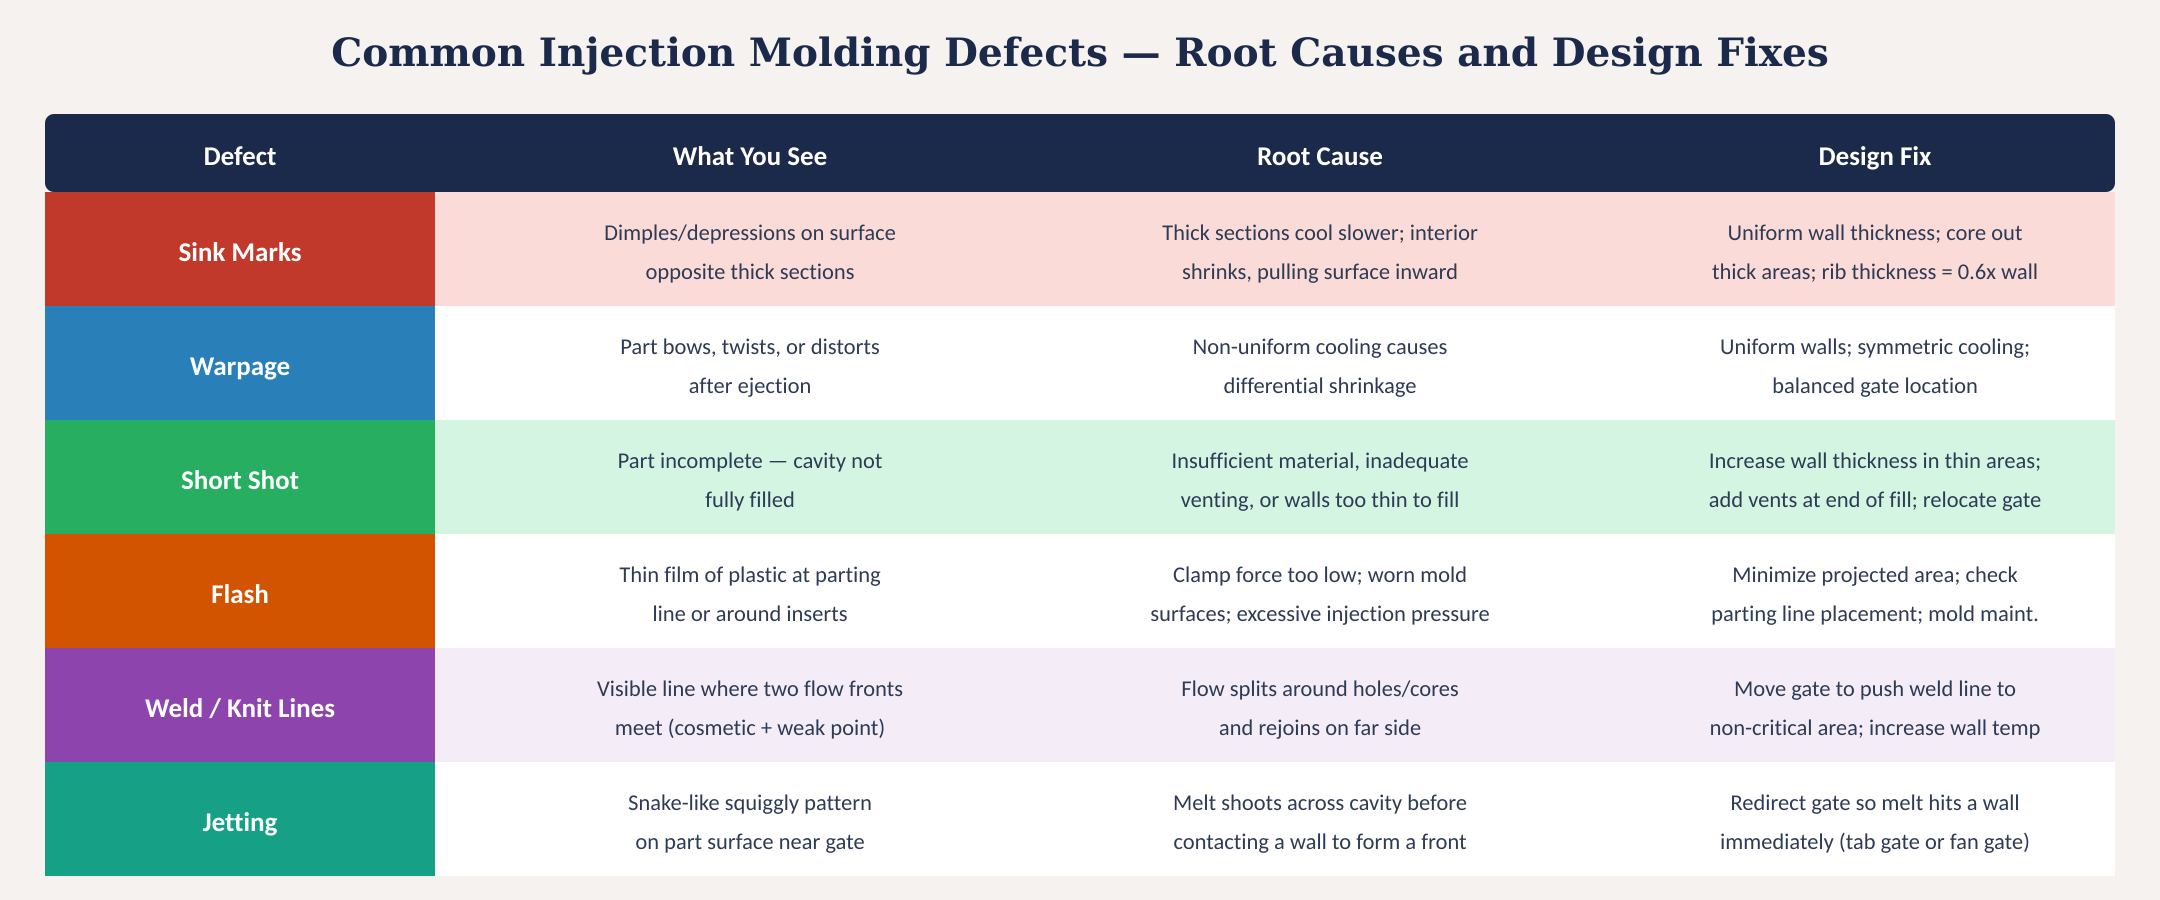
\includegraphics[width=\textwidth]{master_figs/fig_defects.png}
\caption{Six common injection molding defects with visual description, root cause, and design fix.}
\label{fig:defects}
\end{figure}

\begin{table}[htbp]
\centering\small
\begin{tabularx}{\textwidth}{l l X X}
  \toprule
  \textbf{Defect} & \textbf{What You See} & \textbf{Root Cause} & \textbf{Design Fix} \\
  \midrule
  Sink marks & Dimples opposite thick sections & Thick areas cool slowly, interior shrinks & Uniform walls; core out; rib = 0.6$\times$ wall \\
  Warpage & Part bows/twists after ejection & Non-uniform cooling $\to$ differential shrinkage & Uniform walls; symmetric cooling; balanced gate \\
  Short shot & Incomplete part & Inadequate venting, thin walls, low pressure & Vent at end of fill; increase thin walls \\
  Flash & Thin film at parting line & Low clamp force, worn mold, high pressure & Minimize projected area; mold maintenance \\
  Weld lines & Visible line where fronts meet & Flow splits around holes/cores & Relocate gate; increase melt temperature \\
  Jetting & Squiggly pattern near gate & Melt shoots across cavity before wall contact & Redirect gate so melt hits a wall immediately \\
  \bottomrule
\end{tabularx}
\caption{Common defects, root causes, and design fixes.}
\end{table}

\begin{tipbox}[Weld Line Strength]
Weld lines retain only 50--90\% of base material strength. If a weld line falls on a load-bearing feature, relocate the gate or add ribs to reinforce. Flow simulation is the primary tool for predicting and relocating weld lines before cutting the mold.
\end{tipbox}


% ══════════════════════════════════════════════════════════════════════

\subsection{Worked DFM Example: Sensor Enclosure}
\textbf{Requirements}: outdoor IP65 enclosure for GreenShield controller, ABS material, holds PCB (60$\times$40\,mm) and two cable glands.

\textbf{Design decisions}:
\begin{itemize}[nosep,leftmargin=1.5em]
\item \textbf{Wall thickness}: 2.0\,mm uniform (ABS range: 1.5--3.5\,mm). Adequate for IP65 with gasket groove.
\item \textbf{Draft}: \ang{2} on all external walls. C-1 matte finish; no additional texture draft needed.
\item \textbf{Ribs}: four internal ribs at 1.2\,mm thick ($0.6 \times 2.0$), 6.0\,mm tall ($3 \times 2.0$), connecting the PCB mounting bosses to the walls. Base radius 0.5\,mm.
\item \textbf{Bosses}: four PCB mounting bosses, OD = 6.0\,mm ($2.5 \times 2.4$\,mm screw), wall = 1.2\,mm, height = 10\,mm. Each connected to nearest wall by a rib.
\item \textbf{Radii}: all inside corners 1.0\,mm ($0.5 \times 2.0$\,mm wall). Outside corners 3.0\,mm (inside + wall).
\item \textbf{Sealing}: 1.5\,mm wide $\times$ 1.0\,mm deep O-ring groove around the lid perimeter. Silicone O-ring (cord dia.\ 1.5\,mm, compressed to 75\% = 1.0\,mm groove depth).
\item \textbf{Gate}: edge gate on the bottom face (non-cosmetic), at the thickest section near a rib intersection.
\item \textbf{Parting line}: at the lid/base junction (natural split).
\end{itemize}

\section{Tooling and Economics}
\label{sec:tooling}
% ══════════════════════════════════════════════════════════════════════

\begin{figure}[htbp]
\centering
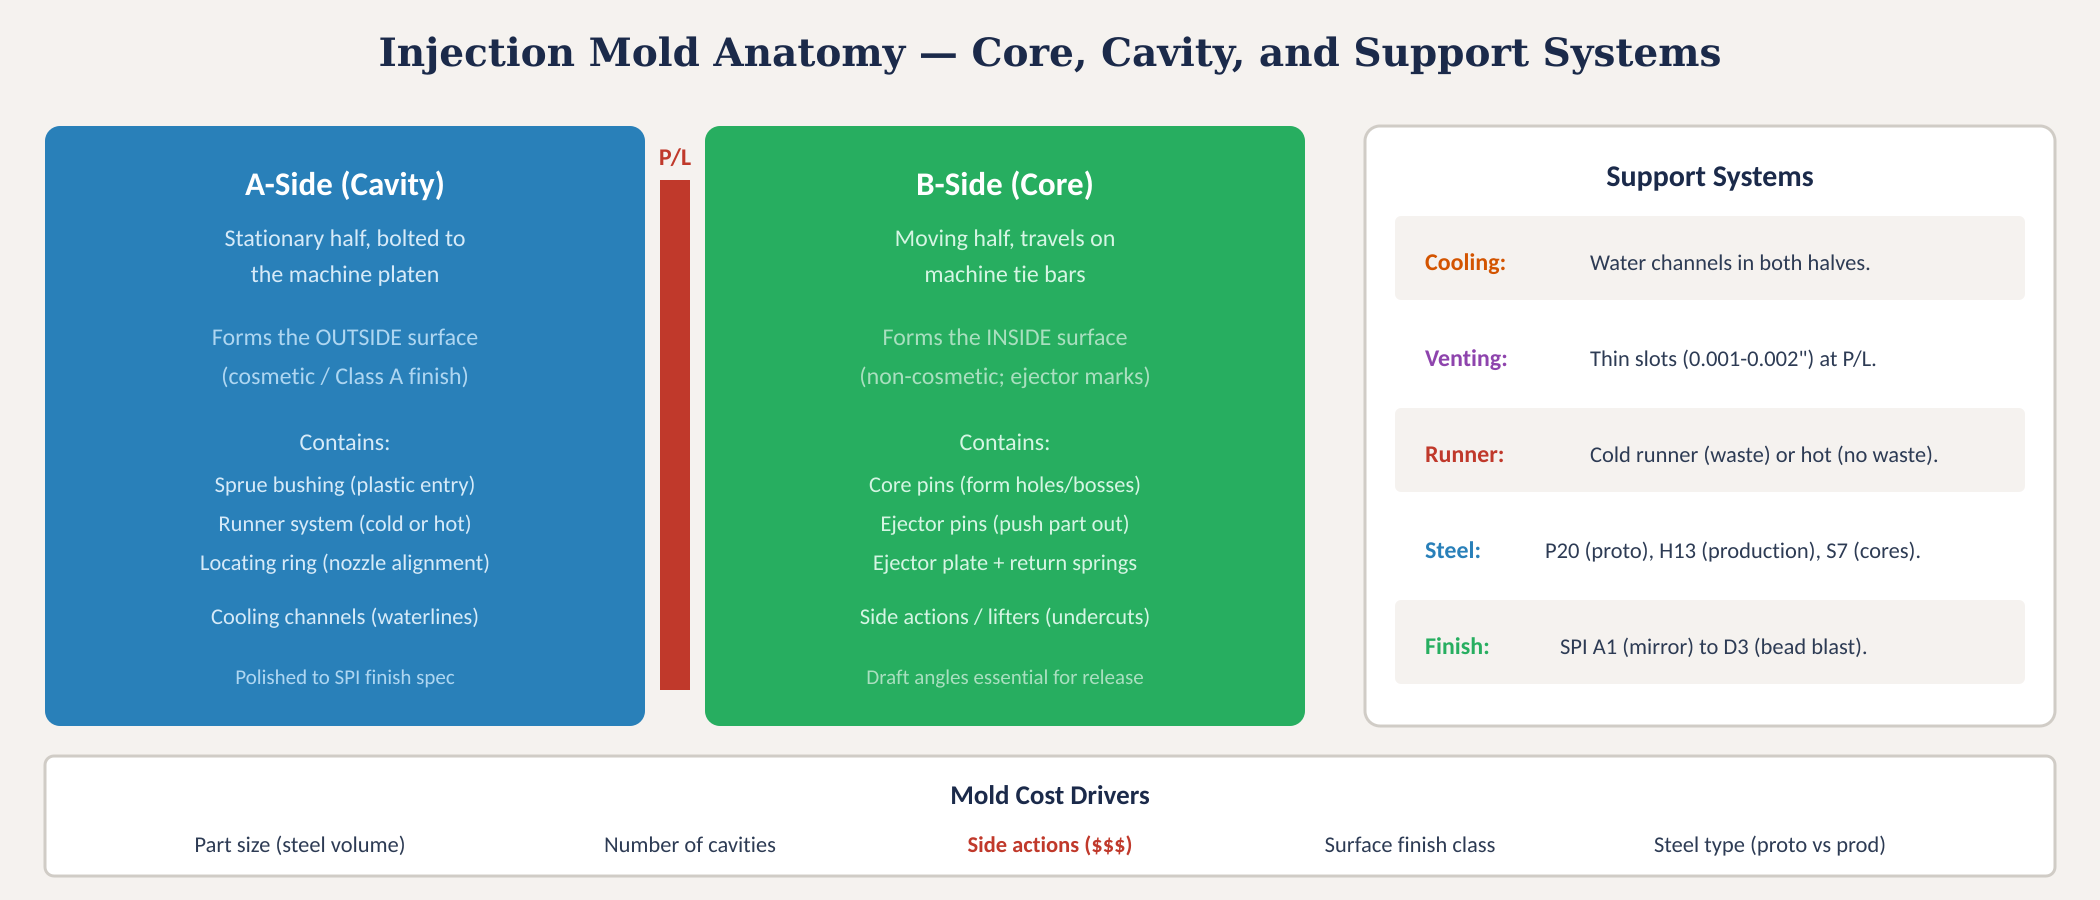
\includegraphics[width=\textwidth]{master_figs/fig_mold_anatomy.png}
\caption{Mold anatomy: A-side (cavity), B-side (core), parting line, support systems, and cost drivers.}
\label{fig:mold}
\end{figure}

\subsection{Mold Construction}

The \textbf{A-side} (cavity) forms the cosmetic outside surface. It contains the sprue bushing, runner system, and locating ring. Surfaces are polished to SPI specifications (A-1 mirror to D-3 bead blast). The \textbf{B-side} (core) forms the inside surface and contains core pins, ejector pins, ejector plates, and side actions. The parting line between the halves leaves a witness mark on the part.

\textbf{Support systems}: cooling channels (water lines in both halves; conformal cooling can reduce cycle time 20--40\%), venting (thin slots 0.001--0.002\,in at parting line), runner system (cold runner produces waste; hot runner eliminates waste but costs more), and ejection system (pins, sleeves, blades, stripper plates).

\subsection{Mold Classifications (SPI)}

\begin{table}[htbp]
\centering\small
\begin{tabularx}{\textwidth}{l l l l X}
  \toprule
  \textbf{Class} & \textbf{Steel} & \textbf{Life (cycles)} & \textbf{Cost Range} & \textbf{Use} \\
  \midrule
  105 (Prototype) & Aluminum / soft steel & $<$500 & \$5K--\$15K & Design validation, pilot runs \\
  104 (Low Prod.) & P20 pre-hardened & $<$100K & \$15K--\$50K & Low volume, bridge tooling \\
  103 (Med. Prod.) & H13 hardened & $<$500K & \$30K--\$80K & Medium-volume production \\
  101 (High Prod.) & Premium hardened & 1M+ & \$50K--\$200K+ & High-volume, long-life production \\
  \bottomrule
\end{tabularx}
\caption{SPI mold classifications.}
\end{table}

\begin{tipbox}[Rapid Tooling: The Bridge Between 3D Printing and Production]
For post-graduation startups or senior design continuations, \textbf{Class~105 prototype molds} (aluminum, \$5K--15K) offer a middle path. Services like Protolabs and Xometry CNC-machine aluminum molds in 10--15 business days for short runs (50--500 parts). This lets you validate DFM, test real injection-molded material properties, and produce enough units for beta testing without committing to a \$50K production mold. Design your MEGN~301 parts with full DFM rules even when 3D printing; if the design is DFM-compliant, the transition to rapid tooling requires only mold design, not part redesign.
\end{tipbox}

\begin{equation}
  C_{\text{part}} = C_{\text{material}} + C_{\text{cycle}} + C_{\text{tooling,amortized}}
\end{equation}

where $C_{\text{material}} = \text{weight} \times \text{resin cost}$, $C_{\text{cycle}} = \text{cycle time} \times \text{machine rate} / 3600$, and $C_{\text{tooling}} = \text{mold cost} / \text{expected lifetime parts}$.

\textbf{Example} (small ABS enclosure, 30\,g): Material: \$0.06. Cycle (25\,s at \$60/hr): \$0.42. Tooling (\$25K amortized over 50K parts): \$0.50. \textbf{Total: \$0.98/part}. At 500K parts, tooling drops to \$0.05/part, total \$0.53/part.

Injection molding breaks even versus 3D printing at approximately 100--500 parts depending on part size and complexity. Below that, 3D printing is cheaper; above it, injection molding wins dramatically.




\section{Warpage}
Warpage is dimensional distortion that occurs after ejection. It is caused by differential shrinkage: when different regions of the part cool at different rates or have different molecular orientations, they shrink by different amounts, creating internal stresses that bow or twist the part.

\subsection{Causes of Warpage}
\textbf{Differential cooling}: one side of the wall cools faster (e.g., mold steel temperature differs between A-side and B-side). The slow-cooling side shrinks more after ejection, bowing the part toward it. \textbf{Fiber orientation}: glass-filled materials shrink less in the flow direction than across it; 0.3\% vs.\ 0.8\% creates a 0.5\% differential. \textbf{Gate location}: determines flow pattern and therefore orientation pattern. A poorly placed gate creates asymmetric flow that maximizes differential shrinkage.

\subsection{Designing to Minimize Warpage}
\begin{itemize}[nosep,leftmargin=1.5em]
\item Maintain uniform wall thickness ($\pm$10\%).
\item Equalize cooling on both sides (symmetric cooling channels).
\item Use gating that produces symmetric flow.
\item For glass-filled materials, gate at center to produce radial (symmetric) fiber orientation.
\item Add ribs to resist bowing (ribs on the concave side of expected warp).
\end{itemize}

\section{Surface Finish}
\subsection{SPI (PIA) Finish Standards}
Surface finish is specified using SPI (Society of the Plastics Industry, now PIA) standards:

\begin{table}[htbp]\centering\small
\begin{tabularx}{\textwidth}{l l l X}
\toprule
\textbf{Grade} & \textbf{Finish} & \textbf{Ra ($\mu$m)} & \textbf{Method and Application} \\
\midrule
A-1 & Mirror & 0.012 & Diamond buff. Optical lenses, light pipes. \\
A-2 & High gloss & 0.025 & Diamond buff. Cosmetic consumer products. \\
B-1 & Semi-gloss & 0.05 & 600 grit paper. General cosmetic surfaces. \\
C-1 & Matte & 0.35 & 600 stone. Hides sink marks, fingerprints. \\
D-1 & Textured & 1.0 & Dry blast. Grips, non-slip, industrial. \\
D-3 & Rough texture & 3.2 & Coarse blast. Heavily textured panels. \\
\bottomrule
\end{tabularx}
\caption{SPI/PIA mold surface finish standards.}
\end{table}

Higher polish = higher mold cost. C-1 matte is the sweet spot for most student and industrial enclosures; hides minor defects while maintaining a professional appearance.

\subsection{Textured Surfaces and Draft}
Texture creates an effective undercut. Add \ang{1} of additional draft per 0.001\,in (0.025\,mm) of texture depth. A D-1 texture (1.0\,$\mu$m Ra, $\sim$0.001\,in depth) requires \ang{1} extra draft beyond the baseline. Failing to add texture draft causes drag marks during ejection.

\section{Insert Molding and Overmolding\index{overmolding}}
\subsection{Insert Molding}
A pre-formed component (metal insert, PCB, bushing) is placed in the mold before injection. Plastic flows around and bonds to the insert. Use when you need: threaded metal inserts (stronger than threading into plastic), electrical contacts molded into a housing, or reinforcing metal structures embedded in plastic.

Design rules: provide $\geq$1.5\,mm of plastic around the insert, add knurling or grooves for mechanical interlock, preheat metal inserts to reduce thermal shock stress, and ensure the insert is fixtured precisely.

\subsection{Overmolding}
A second material is molded over a previously molded substrate. Two-shot or two-step process. Common application: soft TPE grip over rigid ABS body (power tools, toothbrushes, medical devices). The two materials must be chemically compatible for adhesion. Common pairs: ABS/TPE, PC/TPE, nylon/TPE.

\section{Living Hinges and Snap-Fit Clips}
\subsection{Living Hinges}
A living hinge is a thin, flexible web of plastic that connects two rigid sections, allowing them to flex repeatedly without breaking. \textbf{Polypropylene (PP)} is the only commonly injection-molded material suitable for living hinges; its molecular structure allows millions of flex cycles without fatigue. Design rules: hinge thickness 0.25--0.50\,mm, web length 1.0--1.5\,mm, flex immediately after molding (orients molecules across the hinge, increasing life by $10\times$), and gate so flow is perpendicular to the hinge line.

\begin{tipbox}[Material Matters]
ABS, PC, and nylon all crack at a living hinge within a few cycles. \textbf{Only PP} (and some PE grades) can survive millions of flexes. If your design needs a living hinge, the part must be PP; no exceptions.
\end{tipbox}

\subsection{Snap-Fit Clips}
Cantilever snaps are the most common: a beam deflects during assembly, then locks behind a lip. Design for the allowable strain of your material: 2\% for ABS, 4\% for PP, 1.5\% for PC. Maximum deflection: $y = \epsilon L^2 / (1.5t)$ where $\epsilon$ = allowable strain, $L$ = beam length, $t$ = beam thickness. Include a lead-in angle (30--\ang{45}) for easy assembly and a steeper retaining angle (80--\ang{90}) for secure locking. Snap-fits eliminate screw hardware; a significant DFA (Design for Assembly) advantage.

% ══════════════════════════════════════════════════════════════════════
\section{Artifact Handoff: What This Chapter Supports}
\begin{table}[htbp]\centering\small
\begin{tabularx}{\textwidth}{l X l}
\toprule
\textbf{Artifact} & \textbf{Description} & \textbf{Forward Reference} \\
\midrule
DFM Review & Checklist verification for each molded part & CDR deliverable \\
Material Selection & Resin choice with shrinkage and property data & BOM, tolerance analysis \\
Tooling Estimate & Mold class, cost, and timeline & Budget, schedule \\
\bottomrule
\end{tabularx}
\end{table}

\section{DFM Checklist}
\label{sec:checklist_b}
% ══════════════════════════════════════════════════════════════════════

Review every item before sending your CAD model to a molder.

\begin{enumerate}[leftmargin=1.5em]
  \item Wall thickness uniform ($\pm$10\%)? Within recommended range for material?
  \item Draft angles applied to ALL surfaces parallel to pull direction? Texture draft added?
  \item Ribs at 50--70\% of wall? Height $\leq 3\times$ wall? Base radii present?
  \item Bosses at $2\times$ hole ID? Connected to walls with ribs? Boss wall $\leq 0.6\times$ nominal?
  \item All inside corners radiused (min $0.5\times$ wall)? Outside radius = inside + wall?
  \item Undercuts identified? Side actions justified or redesigned out?
  \item Gate location at thickest section? Not on cosmetic surface?
  \item Parting line location acceptable on finished part?
  \item Ejector pin locations on non-cosmetic surfaces? Adequate draft for release?
  \item Shrinkage accounted for in critical dimensions? Tolerances achievable ($\pm$0.005\,in typical)?
  \item Material selected? Properties verified against operating conditions?
  \item Moldflow or fill analysis run? Weld lines and air traps identified?
\end{enumerate}

\begin{warningbox}[Fix Problems in CAD, Not in Steel]
Fixing a design problem in CAD takes minutes. Finding the same problem after the mold is cut costs \$5,000--\$20,000 in mold modifications and 2--4 weeks of delay. Run this checklist at your CDR before committing to tooling.
\end{warningbox}

\begin{keyconceptbox}[Requirements Mapping: From DFM Rules to Shall-Statements]
Injection molding constraints generate system requirements:
\begin{itemize}[nosep,leftmargin=1.5em]
\item ``Part must survive 1\,m drop onto concrete'' $\to$ MAT-REQ: Material shall have Izod impact $\geq$200\,J/m (ABS or PC/ABS).
\item ``Outdoor enclosure, 5+ year UV exposure'' $\to$ MAT-REQ: Material shall be UV-stabilized or painted.
\item ``Volume 50K units/year'' $\to$ TOOL-REQ: Mold shall be SPI Class~104 (P20 steel, $\leq$100K cycle life).
\item ``Assembly time $<$30\,s'' $\to$ DFA-REQ: Enclosure shall use snap-fit closure (no fasteners). Cantilever strain $\leq$2\% for ABS.
\end{itemize}
\end{keyconceptbox}


% ══════════════════════════════════════════════════════════════════════
\section{Practice Questions}
\label{sec:practice_b}
% ══════════════════════════════════════════════════════════════════════

\subsection{Conceptual Questions}

\begin{enumerate}[leftmargin=1.5em]
  \item Why does cooling time scale with the \emph{square} of wall thickness rather than linearly? How does this affect part cost?

  \item A part has a 4\,mm thick boss connected to a 2\,mm wall. Predict the defect you will see on the surface opposite the boss. What is the design fix?

  \item Explain why a part shrinks onto the core side of the mold during cooling. How does this affect draft angle requirements for the core versus cavity sides?

  \item Your part has a snap hook that creates an undercut on one side. The molder quotes \$18,000 for the side action. Propose two redesign alternatives that might eliminate the side action.

  \item Compare ABS and polypropylene for a consumer electronics enclosure that must accept paint and withstand a 1-meter drop test. Which do you recommend and why?

  \item Why must the gate be placed at the thickest section? What happens if you gate at a thin section instead?

  \item A textured surface (SPI D-2, depth $\approx$ 0.002\,in) on a 3-inch-deep wall currently has \ang{1} of draft. Is this sufficient? If not, what is the correct draft angle?
\end{enumerate}

\subsection{Application / Scenario Questions}

\begin{enumerate}[resume,leftmargin=1.5em]
  \item You are designing a two-piece snap-fit enclosure for an IoT sensor that will be installed outdoors. The enclosure must be IP65, withstand $-20$ to $+60$\,\degC{}, resist UV for 5+ years, and cost under \$3/part at 10,000 units. Select the material, specify wall thickness, describe the snap-fit design, and estimate whether injection molding is economically justified.

  \item Your teammate's CAD model for a motor mount bracket has: 5\,mm walls, zero draft on all vertical surfaces, sharp inside corners, and a boss with OD = 1.5$\times$ hole ID. List every DFM violation, predict the defects that will result from each, and specify the corrected dimensions.

  \item \textbf{Cost analysis}: A part weighs 45\,g in PC/ABS (\$0.003/g). Cycle time is 30\,seconds on a machine at \$75/hr. The mold costs \$35,000. Calculate the total part cost at 5,000, 50,000, and 500,000 units. At what volume does injection molding become cheaper than SLA 3D printing at \$8.50/part?
\end{enumerate}

\subsection{Answers}

\begin{enumerate}[leftmargin=1.5em]
  \item Cooling is a transient heat-conduction problem governed by the Fourier equation. The characteristic time for heat to diffuse through a slab of thickness $t$ scales as $t^2 / \alpha$ where $\alpha$ is thermal diffusivity. Doubling wall thickness from 2\,mm to 4\,mm quadruples cooling time; potentially adding 20--40 seconds per cycle. At a machine rate of \$60/hr, each additional second costs approximately \$0.017/part. Over 100,000 parts, a 20-second cycle-time penalty costs \$17,000.

  \item A sink mark (dimple/depression) on the surface opposite the boss. The 4\,mm boss is twice the 2\,mm wall, creating a thick section that cools more slowly. The interior shrinks and pulls the surface inward. Fix: reduce boss wall to $0.6 \times 2 = 1.2$\,mm (OD = hole ID + 2$\times$1.2\,mm). Connect the boss to the nearest wall with a thin rib.

  \item As plastic cools it contracts volumetrically. The cavity half forms the outside surface, and the part shrinks \emph{away} from it, naturally releasing. The core half forms the inside surface, and the part shrinks \emph{onto} it, gripping tighter as it cools. This means the core side typically needs more draft (\ang{1.5}--\ang{2}) than the cavity side (\ang{0.5}--\ang{1}) to overcome the shrink-grip.

  \item (a) Reorient the snap hook to flex along the mold-open direction; if the hook can deflect during ejection, no side action is needed (the hook ``snaps'' past the mold surface). (b) Replace the snap hook with a separate clip that installs post-molding via a push-fit or ultrasonic weld, eliminating the undercut entirely.

  \item ABS. Both have adequate impact strength, but ABS accepts paint directly (smooth surface, good adhesion) while PP requires flame treatment or specialty primers due to its low surface energy. ABS also has a higher HDT ($\sim$95\,\degC{} versus $\sim$60\,\degC{} for unfilled PP), providing more thermal margin. ABS shrinkage (0.5--0.7\%) is lower and more predictable than PP (1.0--2.5\%), enabling tighter dimensional control for snap-fits and mating features.

  \item Gating at the thickest section ensures that the section that shrinks the most remains connected to the runner for packing pressure the longest. If you gate at a thin section, the thin area freezes first and seals off (``gates off''), cutting the thick section off from packing pressure. The result is severe sink marks and voids in the thick section because the material cannot be replenished as it shrinks.

  \item No. The texture-depth rule requires adding \ang{1} per 0.001\,in of depth. At 0.002\,in depth, add \ang{2} beyond the standard \ang{1} for a total of \ang{3} per side. Without adequate draft, the textured surface acts like sandpaper during ejection, leaving drag marks that ruin the finish and gouge the mold steel.

  \item Material: ASA (acrylic-styrene-acrylonitrile), UV-stable variant of ABS, good impact from $-20$ to $+80$\,\degC{}, IP65-rated with proper gasket design, paintable if needed. Wall thickness: 2.0\,mm nominal (meets structural requirements, enables IP65 with perimeter gasket groove). Snap-fit: cantilever snaps along the mold-open axis (no side action), 2\% max strain for ASA, designed with \ang{1.5} draft. Economics: at 10,000 units with a Class~104 mold (\$25K), tooling amortization is \$2.50/part. Material (20\,g $\times$ \$0.003): \$0.06. Cycle (20\,s at \$60/hr): \$0.33. Total: $\sim$\$2.89/part, under the \$3 target. Injection molding is justified.

  \item Violations and fixes: (a) 5\,mm walls are too thick for any common plastic; excessive cooling time, sink marks, voids. Fix: core out to 2\,mm uniform walls, add ribs for stiffness. (b) Zero draft on all vertical surfaces; parts will stick, ejector damage, mold wear. Fix: add minimum \ang{1} per side to all surfaces parallel to pull. (c) Sharp inside corners; stress concentrations ($3\times$ multiplier), impeded flow. Fix: add $R = 0.5 \times 2 = 1$\,mm fillet to all inside corners; outside radius = $1 + 2 = 3$\,mm. (d) Boss OD at $1.5\times$ hole ID is too thin-walled, creating a thick ring that sinks. Fix: increase OD to $2.0\times$ hole ID. Predicted defects: sink marks everywhere (thick walls + oversized boss), warpage (non-uniform cooling from variable thickness), ejection damage (no draft), cracking at corners under load (no radii).

  \item Material: $45 \times 0.003 = \$0.135$/part. Cycle: $30/3600 \times 75 = \$0.625$/part. These are constant.

  At 5,000 parts: tooling $= 35000/5000 = \$7.00$/part. Total: $\$7.76$/part.

  At 50,000 parts: tooling $= 35000/50000 = \$0.70$/part. Total: $\$1.46$/part.

  At 500,000 parts: tooling $= 35000/500000 = \$0.07$/part. Total: $\$0.83$/part.

  Break-even vs.\ SLA at \$8.50/part: solve $0.135 + 0.625 + 35000/n = 8.50$. $35000/n = 7.74$. $n = 4,522$ parts. Above $\sim$4,500 parts, injection molding is cheaper.
\end{enumerate}


% ══════════════════════════════════════════════════════════════════════




\subsection{Application / Scenario Questions}
\begin{enumerate}[leftmargin=1.5em, start=7]
\item You are designing an outdoor sensor enclosure in ABS. The enclosure must be IP65 (dust-tight, water-jet resistant). Specify: wall thickness, draft angles, sealing method, and surface finish. Justify each choice.
\item A client asks you to injection mold a part with a living hinge. They want to use ABS because it matches the rest of their product line. What do you tell them?
\item Your injection-molded part has sink marks opposite the boss locations. The bosses are 3.0\,mm wall in a part with 2.0\,mm nominal wall. What is wrong, and how do you fix it?
\end{enumerate}

\subsection{Answers to Application Questions}
\begin{enumerate}[leftmargin=1.5em, start=7]
\item Wall: 2.0\,mm nominal (meets structural, enables IP65 with perimeter gasket groove). Draft: \ang{2} standard on all external walls; add \ang{1} per 0.001\,in of texture depth if textured. Sealing: silicone O-ring in a groove on the lid mating surface (not adhesive or gasket tape). Surface: C-1 matte (hides minor defects, professional appearance, reduces mold cost vs.\ polish). Internal surfaces: D-1 textured (hides ejector pin marks).
\item ABS cannot survive living hinge cycles; it will crack within 1--5 flexes. Only PP (and some PE) can form living hinges that last millions of cycles. Options: (a) redesign the part in PP; (b) use a separate PP living hinge piece bonded/overmolded to the ABS body; (c) replace the living hinge with a mechanical hinge (pin + knuckle) that can be molded in ABS.
\item Boss wall = 3.0\,mm vs.\ 2.0\,mm nominal = 150\% of wall thickness. This thick section cools slowly, creating a void that pulls the surface inward (sink mark). Fix: reduce boss wall to $0.6 \times 2.0 = 1.2$\,mm (60\% of nominal). If the boss needs more material for screw engagement, connect it to the nearest wall with a rib (rib at 60\% wall = 1.2\,mm).
\end{enumerate}

